\subsection{Parking Lot Generation}

The ParkingGenerator function takes a plot and its underlying terrain as input, and produces a parking lot as output (see Table~\ref{table:parking}).
This generator in particular is responsible for filling roughly ten percent of the generated cities with parking lots, a percentage based on research conducted in Phoenix,~AZ~\cite{parking_percent}.

\begin{table}[H]
   \centering
   \begin{tabular}{lllll}
     \textbf{Input}                           &               & \textbf{Function}            &               & \textbf{Output}         \\
     \midrule
     \textit{Plot, Terrain}                   & $\rightarrow$ & \textbf{ParkingGenerator}       & $\rightarrow$ & \textit{Parking lot}           \\
     \bottomrule
   \end{tabular}

   \caption{Definition of the ParkingGenerator function which is responsible for generating parking lots.}
   \label{table:parking}
 \end{table}
 \vspace{-0.4cm}

One approach considered for the generation of parking lots was to simply cover areas with textures.
This would have been a straightforward option to implement, but it was found that it offers little alternatives for modification.
For example, the shape of the entire parking lot as well as the size of the individual parking spaces would be difficult to adjust afterwards using this approach.
Furthermore, using a mesh with one texture applied to it would remove the possibility of scaling the size of the parking spaces within the mesh without scaling the mesh itself.
As every other generator provides fully scalable content, it would be inconvenient for the ParkingGenerator to be any different.

Another approach was to generate each line in the parking area individually. 
This was the initial approach that was used in the application, but was changed due to performance concerns when dealing with massive amounts of line objects.

The final approach was a combination of these two methods.
The first step of this approach is to fill the plot with asphalt, but this is not an easy task.
This could be achieved by projecting an asphalt mesh onto the plot, however this mesh would need to be perfectly aligned with the terrain mesh.
This was solved by writing an algorithm that essentially cut out a portion of the terrain mesh in the shape of the plot then slightly offsetting it upwards to avoid overlapping triangles with the terrain. (See Figure~\ref{fig:methods_parking_terrain_projector}).
With this method, the mesh would never clip with the terrain.

\begin{figure}[H]
  \centering

  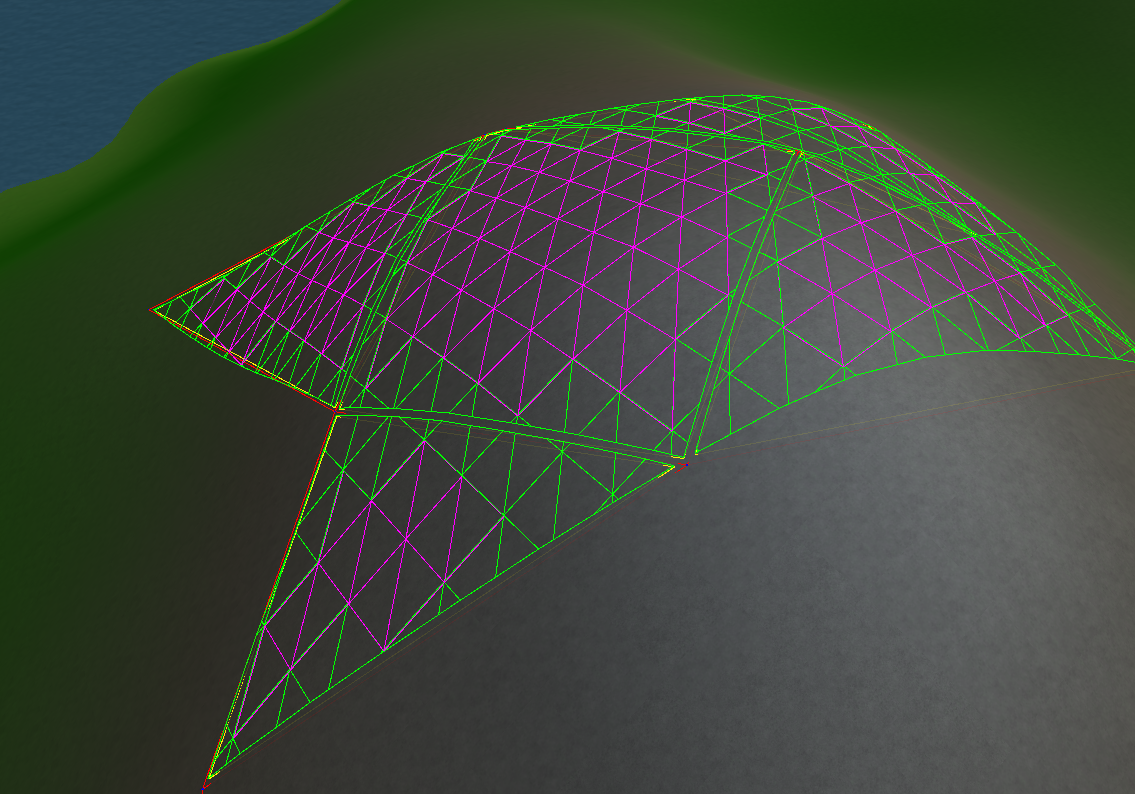
\includegraphics[width=0.8\textwidth]{figure/methods/terrain_projector}
  \caption{Mesh projected onto the terrain.}

  \label{fig:methods_parking_terrain_projector}
\end{figure}

The second step is to place parking lots in suitable locations within the plot.
This was done using a function to approximate the largest rectangle inside a polygon which finds a suitable rectangle to generate parking lots in.
Based on the size of the approximated rectangle, the algorithm generates as many rows of parking lots as it can fit.
Each row contains a quad that is projected onto the terrain with a transparent texture where only the white parking lot lines are opaque.
By modifying the UV coordinates of the quad, the texture can be repeated and scaled to any desired size. 
The plot is also given a margin around it to make sure there is enough space around the parking lots for cars to get in and out of the parking area.

The idea behind the final approach came from the observation that parking lots tend to follow a rectangular shape (see Figure~\ref{fig:parkings}).
Of course, this shape does not cover all types of parking lot, but it seemed like a reasonable scope for this project.

\begin{figure}[H]
  \centering
  \begin{subfigure}[b]{0.55\textwidth}
    \frame{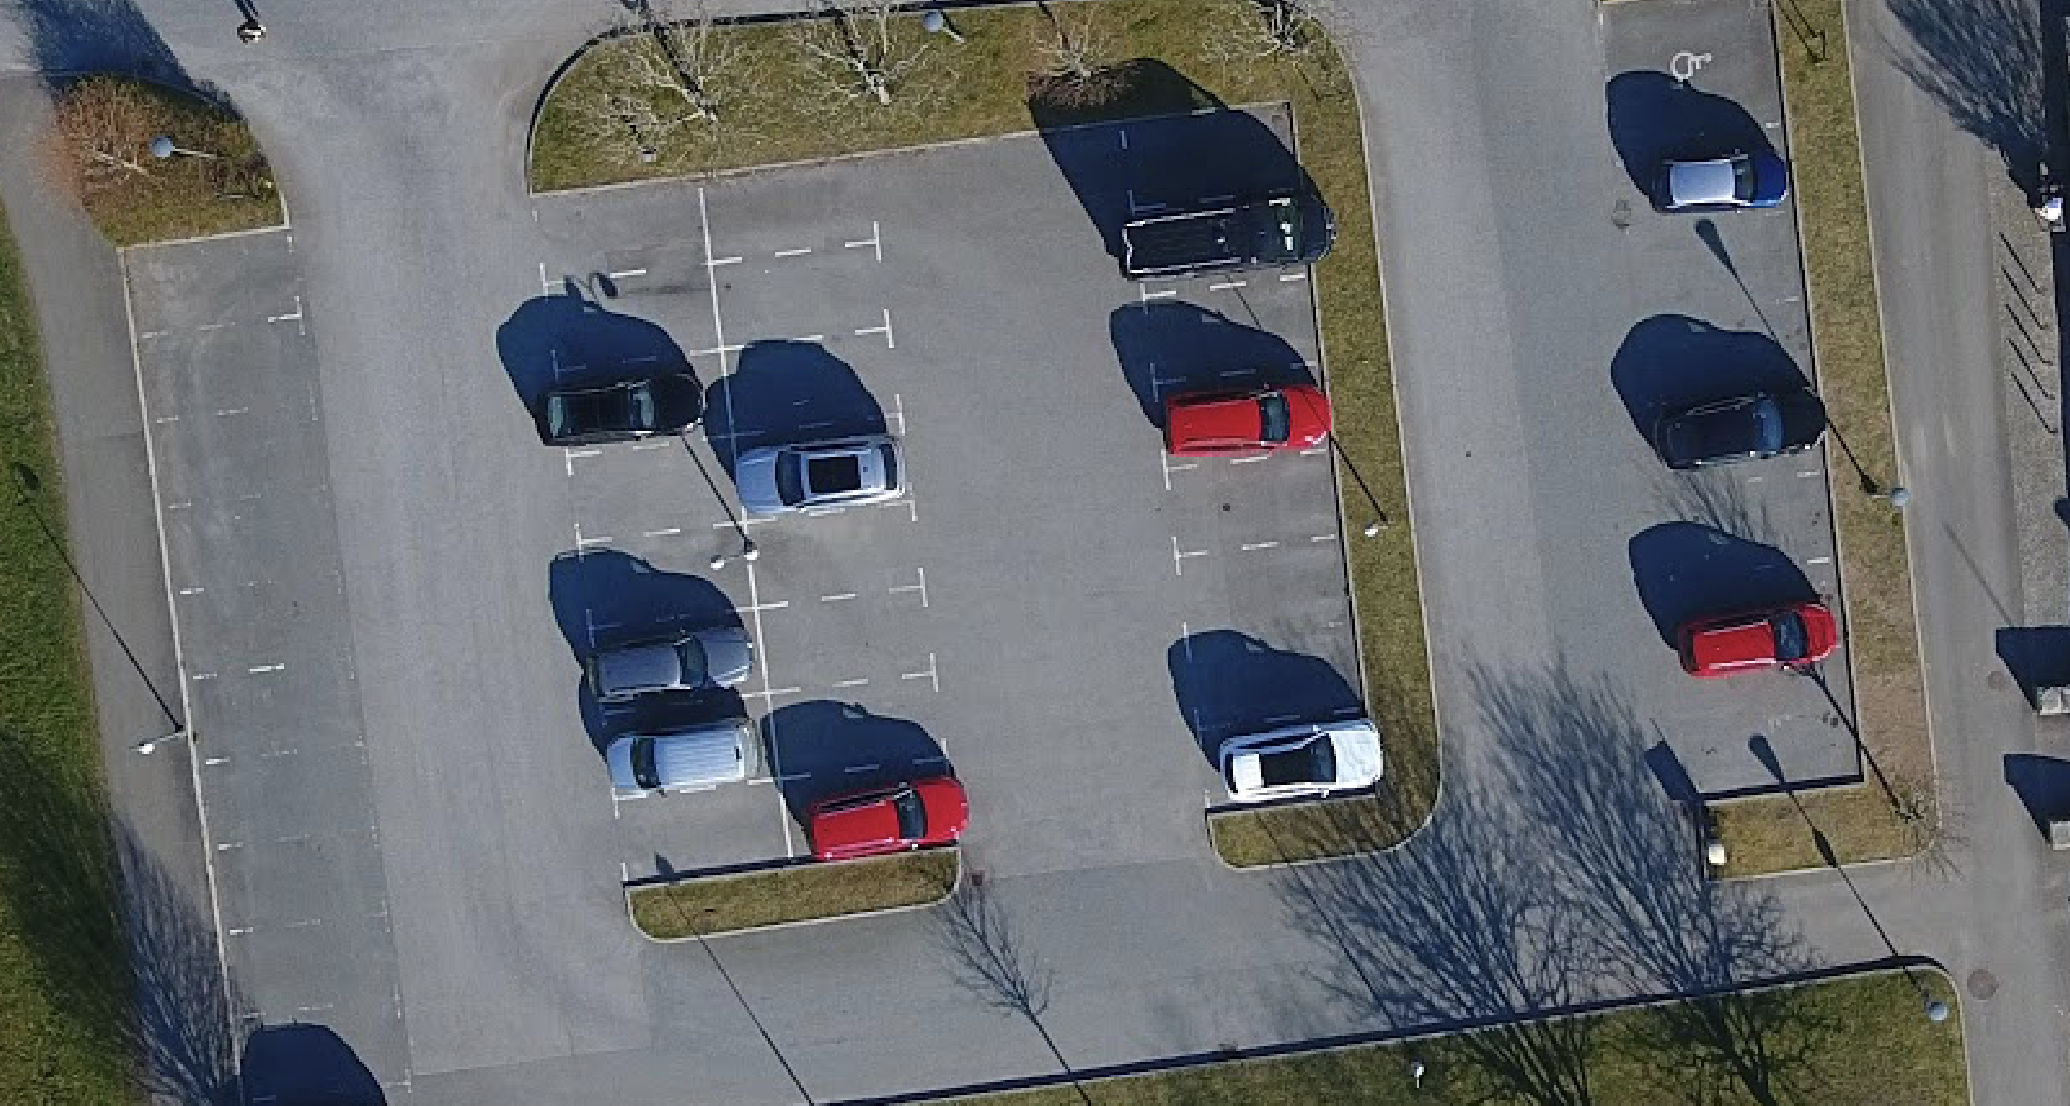
\includegraphics[width=\textwidth]{figure/methods/parking/real1}}
  \end{subfigure}
  \quad
  \begin{subfigure}[b]{0.335\textwidth}
    \frame{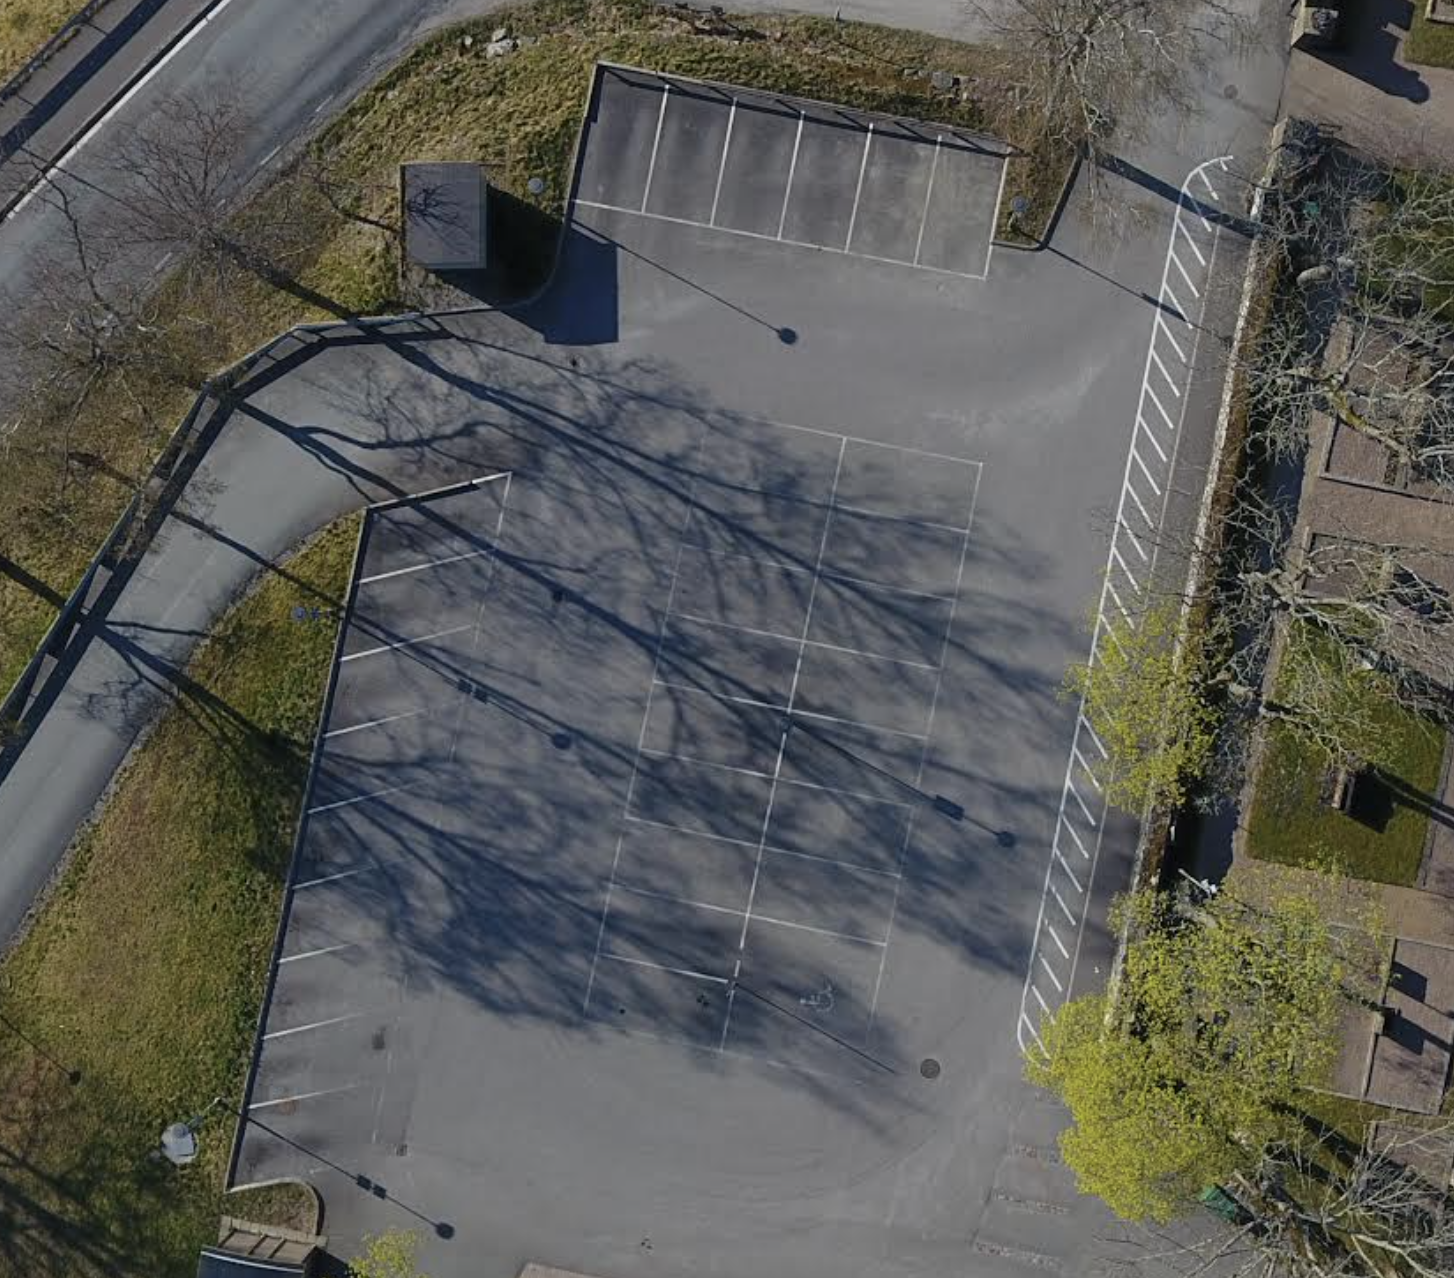
\includegraphics[width=\textwidth]{figure/methods/parking/real2}}
  \end{subfigure}
  \caption{Two examples of parking lots with rectangular shapes. The photos were taken by the project group using a drone.}
  \label{fig:parkings}
\end{figure}
